\begin{figure}
  \centering
    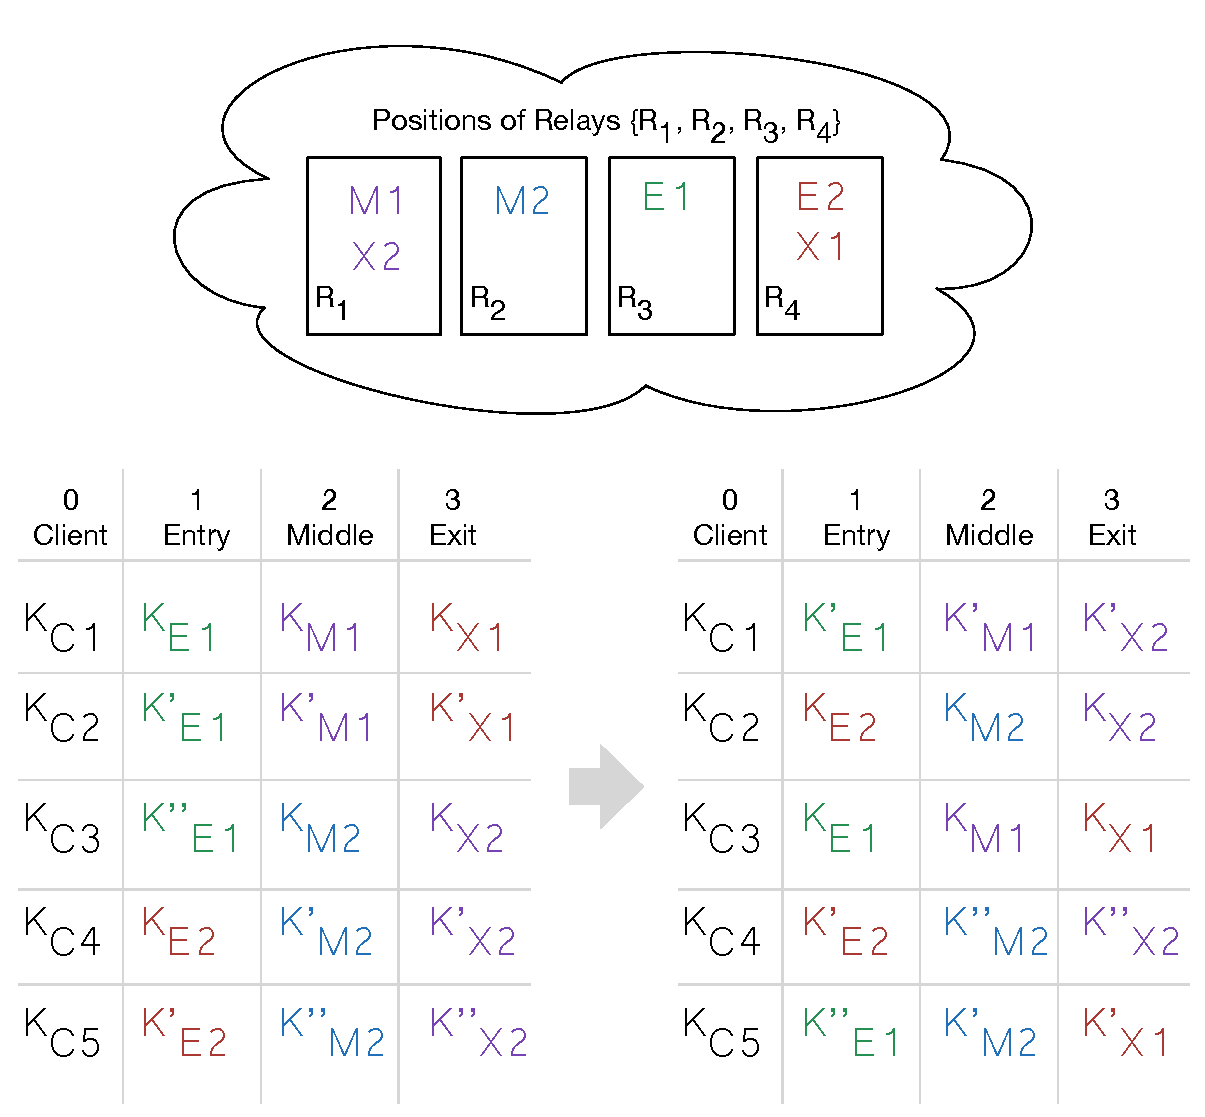
\includegraphics[scale=.6]{shuffle_total.pdf}
  \caption{
    Example matrix shuffle with 5 clients ($C_1$, $C_2$, $C_3$, $C_4$ and $C_5$) 
    and 4 relays (purple, blue, green, red). Each relay $R_i$ generates a number 
    of public keys $K_p^i$ for each circuit position $p \in {E, M, X}$, as 
    instructed by its assignment server. Here, each client $C_j$ is assigned the 
    circuit represented by the $j^{th}$ row of the shuffled matrix. 
  }
  \label{figure:shuffle}
\end{figure}